\section{Spaceteam}

\begin{figure}[h!]
    \centering
    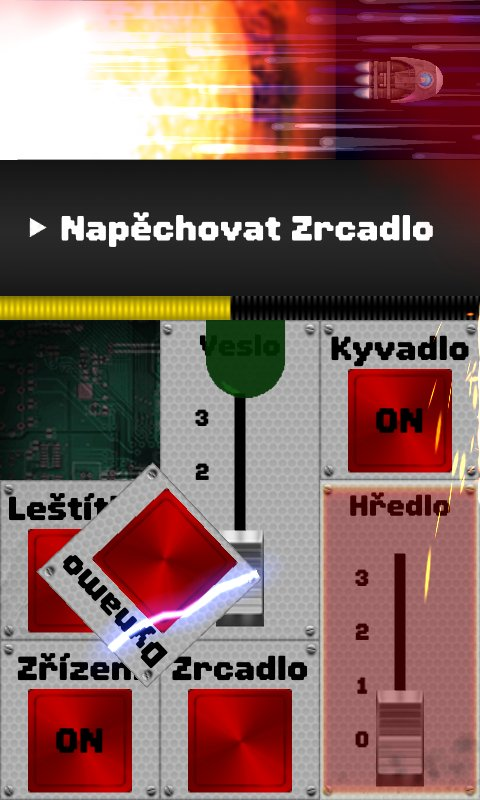
\includegraphics[width=0.5\linewidth]{assets/competitive-apps/spaceteam.jpg}
    \caption{Screenshot hry Spaceteam \cite{henrysmithinc_spaceteam}}
    \label{fig:spaceteam}
\end{figure}

Poslední hra, \emph{Spaceteam}, stojí na rychlosti reakcí a velmi rychlé
komunikaci.
To shrnuje první věta na stránce hry \cite{henrysmithinc_spaceteam}
v obchodě Google Play: \uv{Mačkáš rád tlačítka a řveš na své kamarády?}

Herní plocha je plná náhodných tlačítek, přepínačů, posouvátek a dalších věcí,
které dohromady tvoří ovládací prvky hry.
Každému hráči přichází postupně do zařízení série příkazů,
které cílí na určitou interakci s ovládacími prvky.

Hra je rozdělena na herní kola.
Každé herní kolo má vlastní množinu ovládacích prvků a příkazů.

Zapeklitost komunikace spočívá v tom,
že příkazy se netýkají pouze prvků na nadaném zařízení,
ale i prvků ze zařízení ostatních hráčů.
Některé příkazy také cílí na všechny hráče.
Příkladem takévého příkazu je například zatřesení všemi zařízeními najednou.

Každý chybný krok je penalizován.
Penalizace se postupně projevuje například zhoršením přístupnosti k ovládacím
prvkům.
Cílem hry je dostat se přes co nejvíce herních kol.
Po skončení hry následuje shrnující statistika a ocenění jednotlivých hráčů.

\subsection*{Klady}

\begin{itemize}
    \item UI úvodní obrazovky a přihlašování do hry vypadá velmi efektně.
    \item Tlačítka i příkazy obsahují řadu technologických pojmů,
což dodává hře na správné atmosféře.
    \item Finální ocenění hráčů působí vřelým dojmem.
\end{itemize}

\subsection*{Zápory}

\begin{itemize}
    \item Herní obrazovka má poněkud zastaralé, až nevkusné, prvky.
    \item Hra probíhá až příliš rychle.
Nutno přiznat, že tento fakt není nutně nevýhoda,
avšak ubírá to na prvku kvalitnější komunikace.
    \item Hra nemá možnost přihlášení,
a tedy shromažďování a uchovávání statistik.
\end{itemize}
